\documentclass[10pt,xcolor=svgnames]{beamer} %Beamer
\usepackage{palatino} %font type
\usefonttheme{metropolis} %Type of slides
\usefonttheme[onlymath]{serif} %font type Mathematical expressions
\usetheme[titleformat frame=smallcaps]{metropolis} %This adds a bar at the beginning of each section.
% \usetheme[progressbar=frametitle,titleformat frame=smallcaps,numbering=counter]{metropolis}
% \useoutertheme[subsection=false]{miniframes} %Circles in the top of each frame, showing the slide of each section you are at

\usepackage{appendixnumberbeamer} %enumerate each slide without counting the appendix
% \setbeamercolor{progress bar}{fg=Maroon!70!Coral} %These are the colours of the progress bar. Notice that the names used are the svgnames
\setbeamercolor{title separator}{fg=DarkSalmon} %This is the line colour in the title slide
\setbeamercolor{structure}{fg=black} %Colour of the text of structure, numbers, items, blah. Not the big text.
\setbeamercolor{normal text}{fg=black!87} %Colour of normal text
\setbeamercolor{alerted text}{fg=DarkRed!60!Gainsboro} %Color of the alert box
\setbeamercolor{example text}{fg=Maroon!70!Coral} %Colour of the Example block text


\setbeamercolor{palette primary}{bg=NavyBlue!50!DarkOliveGreen, fg=white} %These are the colours of the background. Being this the main combination and so one. 
\setbeamercolor{palette secondary}{bg=NavyBlue!50!DarkOliveGreen, fg=white}
\setbeamercolor{palette tertiary}{bg=NavyBlue!40!Black, fg= white}
\setbeamercolor{section in toc}{fg=NavyBlue!40!Black} %Color of the text in the table of contents (toc)

\usepackage[utf8]{inputenc}
% \usepackage{amsmath,amssymb}
\usepackage[Symbol]{upgreek}
\usepackage{newtxmath}
% \usepackage{slashed}
% \usepackage[capitalise,noabbrev]{cleveref}
% \usepackage{relsize}
% \usepackage{caption}
% \usepackage{subcaption}
\usepackage{multicol}
% \usepackage{booktabs}
% \usepackage[scale=2]{ccicons}
% \usepackage{pgfplots}
% \usepgfplotslibrary{dateplot}
% \usepackage{geometry}
% \usepackage{xspace}
% \usepackage{comment}
% \usepackage{ucs}
% \usepackage{bbm}
\usepackage[style=verbose,backend=biber]{biblatex}
\addbibresource{bib.bib}
\usepackage[greek,english]{babel}
\usepackage{newunicodechar}
% \usepackage{polytable}


\newcommand{\themename}{\textbf{\textsc{bluetemp}\xspace}}%metropolis}}\xspace}

\newcommand{\awa}[2]{\mathrlap{#2}\phantom{#1}} % as wide as
\newcommand{\aha}[2]{\smash{\parbox{\linewidth}{#2}}\phantom{\parbox{\linewidth}{#1}}} % as high as
\newcommand{\parl}[1]{\parbox{\linewidth}{#1}} % as high as

\newcommand{\mi}[1]{\ensuremath{\mathit{#1}}}

\newunicodechar{→}{\ensuremath{\mathord{\rightarrow}}}
\newunicodechar{⇒}{\ensuremath{\Rightarrow}}
\newunicodechar{⊢}{\ensuremath{\vdash}}
\newunicodechar{∀}{\ensuremath{\forall}}
\newunicodechar{ℕ}{\ensuremath{\mathbb{N}}}
\newunicodechar{ƛ}{\ensuremath{\lambdaslash}}
\newunicodechar{Γ}{\ensuremath{\varGamma}}
\newunicodechar{Δ}{\ensuremath{\varDelta}}
\newunicodechar{∋}{\ensuremath{\ni}}
\newunicodechar{μ}{\ensuremath{\mu}}
\newunicodechar{α}{\ensuremath{\alpha}}
\newunicodechar{ρ}{\ensuremath{\rho}}
\newunicodechar{σ}{\ensuremath{\sigma}}
\newunicodechar{τ}{\ensuremath{\tau}}
\newunicodechar{·}{\ensuremath{\mathord\cdotp}}
\newunicodechar{₁}{\ensuremath{_1}}
\newunicodechar{₂}{\ensuremath{_2}}
\newunicodechar{×}{\ensuremath{\times}}
\newunicodechar{ᵈ}{\ensuremath{^d}}
\newunicodechar{ω}{\ensuremath{\omega}}
\newunicodechar{λ}{\ensuremath{\lambda}}
\newunicodechar{▪}{\ensuremath{\blacksquare}}
\newunicodechar{‵}{\ensuremath{\mathord{^\backprime}}}
\newunicodechar{∷}{\ensuremath{::}}
\newunicodechar{∗}{\ensuremath{\mathord\ast}}
\newunicodechar{ℓ}{\ensuremath{\ell}}

%% ODER: format ==         = "\mathrel{==}"
%% ODER: format /=         = "\neq "
%
%
\makeatletter
\@ifundefined{lhs2tex.lhs2tex.sty.read}%
  {\@namedef{lhs2tex.lhs2tex.sty.read}{}%
   \newcommand\SkipToFmtEnd{}%
   \newcommand\EndFmtInput{}%
   \long\def\SkipToFmtEnd#1\EndFmtInput{}%
  }\SkipToFmtEnd

\newcommand\ReadOnlyOnce[1]{\@ifundefined{#1}{\@namedef{#1}{}}\SkipToFmtEnd}
\usepackage{amstext}
\usepackage{amssymb}
\usepackage{stmaryrd}
\DeclareFontFamily{OT1}{cmtex}{}
\DeclareFontShape{OT1}{cmtex}{m}{n}
  {<5><6><7><8>cmtex8
   <9>cmtex9
   <10><10.95><12><14.4><17.28><20.74><24.88>cmtex10}{}
\DeclareFontShape{OT1}{cmtex}{m}{it}
  {<-> ssub * cmtt/m/it}{}
\newcommand{\texfamily}{\fontfamily{cmtex}\selectfont}
\DeclareFontShape{OT1}{cmtt}{bx}{n}
  {<5><6><7><8>cmtt8
   <9>cmbtt9
   <10><10.95><12><14.4><17.28><20.74><24.88>cmbtt10}{}
\DeclareFontShape{OT1}{cmtex}{bx}{n}
  {<-> ssub * cmtt/bx/n}{}
\newcommand{\tex}[1]{\text{\texfamily#1}}	% NEU

\newcommand{\Sp}{\hskip.33334em\relax}


\newcommand{\Conid}[1]{\mathit{#1}}
\newcommand{\Varid}[1]{\mathit{#1}}
\newcommand{\anonymous}{\kern0.06em \vbox{\hrule\@width.5em}}
\newcommand{\plus}{\mathbin{+\!\!\!+}}
\newcommand{\bind}{\mathbin{>\!\!\!>\mkern-6.7mu=}}
\newcommand{\rbind}{\mathbin{=\mkern-6.7mu<\!\!\!<}}% suggested by Neil Mitchell
\newcommand{\sequ}{\mathbin{>\!\!\!>}}
\renewcommand{\leq}{\leqslant}
\renewcommand{\geq}{\geqslant}
\usepackage{polytable}

%mathindent has to be defined
\@ifundefined{mathindent}%
  {\newdimen\mathindent\mathindent\leftmargini}%
  {}%

\def\resethooks{%
  \global\let\SaveRestoreHook\empty
  \global\let\ColumnHook\empty}
\newcommand*{\savecolumns}[1][default]%
  {\g@addto@macro\SaveRestoreHook{\savecolumns[#1]}}
\newcommand*{\restorecolumns}[1][default]%
  {\g@addto@macro\SaveRestoreHook{\restorecolumns[#1]}}
\newcommand*{\aligncolumn}[2]%
  {\g@addto@macro\ColumnHook{\column{#1}{#2}}}

\resethooks

\newcommand{\onelinecommentchars}{\quad-{}- }
\newcommand{\commentbeginchars}{\enskip\{-}
\newcommand{\commentendchars}{-\}\enskip}

\newcommand{\visiblecomments}{%
  \let\onelinecomment=\onelinecommentchars
  \let\commentbegin=\commentbeginchars
  \let\commentend=\commentendchars}

\newcommand{\invisiblecomments}{%
  \let\onelinecomment=\empty
  \let\commentbegin=\empty
  \let\commentend=\empty}

\visiblecomments

\newlength{\blanklineskip}
\setlength{\blanklineskip}{0.66084ex}

\newcommand{\hsindent}[1]{\quad}% default is fixed indentation
\let\hspre\empty
\let\hspost\empty
\newcommand{\NB}{\textbf{NB}}
\newcommand{\Todo}[1]{$\langle$\textbf{To do:}~#1$\rangle$}

\EndFmtInput
\makeatother
%
%
%
%
%
%
% This package provides two environments suitable to take the place
% of hscode, called "plainhscode" and "arrayhscode". 
%
% The plain environment surrounds each code block by vertical space,
% and it uses \abovedisplayskip and \belowdisplayskip to get spacing
% similar to formulas. Note that if these dimensions are changed,
% the spacing around displayed math formulas changes as well.
% All code is indented using \leftskip.
%
% Changed 19.08.2004 to reflect changes in colorcode. Should work with
% CodeGroup.sty.
%
\ReadOnlyOnce{polycode.fmt}%
\makeatletter

\newcommand{\hsnewpar}[1]%
  {{\parskip=0pt\parindent=0pt\par\vskip #1\noindent}}

% can be used, for instance, to redefine the code size, by setting the
% command to \small or something alike
\newcommand{\hscodestyle}{}

% The command \sethscode can be used to switch the code formatting
% behaviour by mapping the hscode environment in the subst directive
% to a new LaTeX environment.

\newcommand{\sethscode}[1]%
  {\expandafter\let\expandafter\hscode\csname #1\endcsname
   \expandafter\let\expandafter\endhscode\csname end#1\endcsname}

% "compatibility" mode restores the non-polycode.fmt layout.

\newenvironment{compathscode}%
  {\par\noindent
   \advance\leftskip\mathindent
   \hscodestyle
   \let\\=\@normalcr
   \let\hspre\(\let\hspost\)%
   \pboxed}%
  {\endpboxed\)%
   \par\noindent
   \ignorespacesafterend}

\newcommand{\compaths}{\sethscode{compathscode}}

% "plain" mode is the proposed default.
% It should now work with \centering.
% This required some changes. The old version
% is still available for reference as oldplainhscode.

\newenvironment{plainhscode}%
  {\hsnewpar\abovedisplayskip
   \advance\leftskip\mathindent
   \hscodestyle
   \let\hspre\(\let\hspost\)%
   \pboxed}%
  {\endpboxed%
   \hsnewpar\belowdisplayskip
   \ignorespacesafterend}

\newenvironment{oldplainhscode}%
  {\hsnewpar\abovedisplayskip
   \advance\leftskip\mathindent
   \hscodestyle
   \let\\=\@normalcr
   \(\pboxed}%
  {\endpboxed\)%
   \hsnewpar\belowdisplayskip
   \ignorespacesafterend}

% Here, we make plainhscode the default environment.

\newcommand{\plainhs}{\sethscode{plainhscode}}
\newcommand{\oldplainhs}{\sethscode{oldplainhscode}}
\plainhs

% The arrayhscode is like plain, but makes use of polytable's
% parray environment which disallows page breaks in code blocks.

\newenvironment{arrayhscode}%
  {\hsnewpar\abovedisplayskip
   \advance\leftskip\mathindent
   \hscodestyle
   \let\\=\@normalcr
   \(\parray}%
  {\endparray\)%
   \hsnewpar\belowdisplayskip
   \ignorespacesafterend}

\newcommand{\arrayhs}{\sethscode{arrayhscode}}

% The mathhscode environment also makes use of polytable's parray 
% environment. It is supposed to be used only inside math mode 
% (I used it to typeset the type rules in my thesis).

\newenvironment{mathhscode}%
  {\parray}{\endparray}

\newcommand{\mathhs}{\sethscode{mathhscode}}

% texths is similar to mathhs, but works in text mode.

\newenvironment{texthscode}%
  {\(\parray}{\endparray\)}

\newcommand{\texths}{\sethscode{texthscode}}

% The framed environment places code in a framed box.

\def\codeframewidth{\arrayrulewidth}
\RequirePackage{calc}

\newenvironment{framedhscode}%
  {\parskip=\abovedisplayskip\par\noindent
   \hscodestyle
   \arrayrulewidth=\codeframewidth
   \tabular{@{}|p{\linewidth-2\arraycolsep-2\arrayrulewidth-2pt}|@{}}%
   \hline\framedhslinecorrect\\{-1.5ex}%
   \let\endoflinesave=\\
   \let\\=\@normalcr
   \(\pboxed}%
  {\endpboxed\)%
   \framedhslinecorrect\endoflinesave{.5ex}\hline
   \endtabular
   \parskip=\belowdisplayskip\par\noindent
   \ignorespacesafterend}

\newcommand{\framedhslinecorrect}[2]%
  {#1[#2]}

\newcommand{\framedhs}{\sethscode{framedhscode}}

% The inlinehscode environment is an experimental environment
% that can be used to typeset displayed code inline.

\newenvironment{inlinehscode}%
  {\(\def\column##1##2{}%
   \let\>\undefined\let\<\undefined\let\\\undefined
   \newcommand\>[1][]{}\newcommand\<[1][]{}\newcommand\\[1][]{}%
   \def\fromto##1##2##3{##3}%
   \def\nextline{}}{\) }%

\newcommand{\inlinehs}{\sethscode{inlinehscode}}

% The joincode environment is a separate environment that
% can be used to surround and thereby connect multiple code
% blocks.

\newenvironment{joincode}%
  {\let\orighscode=\hscode
   \let\origendhscode=\endhscode
   \def\endhscode{\def\hscode{\endgroup\def\@currenvir{hscode}\\}\begingroup}
   %\let\SaveRestoreHook=\empty
   %\let\ColumnHook=\empty
   %\let\resethooks=\empty
   \orighscode\def\hscode{\endgroup\def\@currenvir{hscode}}}%
  {\origendhscode
   \global\let\hscode=\orighscode
   \global\let\endhscode=\origendhscode}%

\makeatother
\EndFmtInput
%

\title{Syntax-Generic Operations, Reflectively Reified}
\author[Name]{Tzu-Chi Lin and Hsiang-Shang Ko} %With inst, you can change the institution they belong
\subtitle{Extended Abstract}
\institute[uni]{Institute of Information Science \\ Academia Sinica, Taiwan}
\date{\today}

\begin{document}
{
	\setbeamercolor{background canvas}{bg=NavyBlue!50!DarkOliveGreen, fg=white}
	\setbeamercolor{normal text}{fg=white}
	\setbeamercovered{transparent}
	\maketitle
}%This is the colour of the first slide. bg= background and fg=foreground

\metroset{titleformat frame=smallcaps} %This changes the titles for small caps

\begin{frame}[fragile]{Outline}
\setbeamertemplate{section in toc}[sections numbered] %This is numbering the sections
\tableofcontents[hideallsubsections] %You can comment this line if you want to show the subsections in the table of contents
\end{frame}

\section{Introduction}

\begin{frame}[fragile]{Motivation}
\emph{Intrinsic typing} is a common pattern that dependently typed programmers use to define $\uplambda$-calculus with De Bruijn indices.
\metroset{block=fill}
\begin{exampleblock}{Example 2.}
	\aha{%
		\begin{hscode}\SaveRestoreHook
\column{B}{@{}>{\hspre}l<{\hspost}@{}}%
\column{3}{@{}>{\hspre}l<{\hspost}@{}}%
\column{10}{@{}>{\hspre}l<{\hspost}@{}}%
\column{E}{@{}>{\hspre}l<{\hspost}@{}}%
\>[B]{}\mathbf{data}\;\Varid{\char95 ⊢\char95 }\;\mathbin{:}\;\Conid{Context}\;\Varid{→}\;\Conid{Type}\;\Varid{→}\;\Conid{Set}\;\mathbf{where}{}\<[E]%
\\
\>[B]{}\hsindent{3}{}\<[3]%
\>[3]{}\Varid{`\char95 }\;{}\<[10]%
\>[10]{}\mathbin{:}\;\Conid{Γ}\;\Varid{∋}\;\Conid{A}\;\Varid{→}\;\Conid{Γ}\;\Varid{⊢}\;\Conid{A}{}\<[E]%
\\
\>[B]{}\hsindent{3}{}\<[3]%
\>[3]{}\Varid{ƛ\char95 }\;{}\<[10]%
\>[10]{}\mathbin{:}\;\Conid{Γ}\;\Varid{,}\;\Conid{A}\;\Varid{⊢}\;\Conid{B}\;\Varid{→}\;\Conid{Γ}\;\Varid{⊢}\;\Conid{A}\;\Varid{⇒}\;\Conid{B}{}\<[E]%
\\
\>[B]{}\hsindent{3}{}\<[3]%
\>[3]{}\Varid{\char95 ·\char95 }\;{}\<[10]%
\>[10]{}\mathbin{:}\;\Conid{Γ}\;\Varid{⊢}\;\Conid{A}\;\Varid{⇒}\;\Conid{B}\;\Varid{→}\;\Conid{Γ}\;\Varid{⊢}\;\Conid{A}\;\Varid{→}\;\Conid{Γ}\;\Varid{⊢}\;\Conid{B}{}\<[E]%
\\
\>[B]{}\hsindent{3}{}\<[3]%
\>[3]{}\Varid{`zero}\;{}\<[10]%
\>[10]{}\mathbin{:}\;\Conid{Γ}\;\Varid{⊢}\;\Varid{`ℕ}{}\<[E]%
\\
\>[B]{}\hsindent{3}{}\<[3]%
\>[3]{}\Varid{`suc\char95 }\;{}\<[10]%
\>[10]{}\mathbin{:}\;\Conid{Γ}\;\Varid{⊢}\;\Varid{`ℕ}\;\Varid{→}\;\Conid{Γ}\;\Varid{⊢}\;\Varid{`ℕ}{}\<[E]%
\\
\>[B]{}\hsindent{3}{}\<[3]%
\>[3]{}\Varid{case}\;{}\<[10]%
\>[10]{}\mathbin{:}\;\Conid{Γ}\;\Varid{⊢}\;\Varid{`ℕ}\;\Varid{→}\;\Conid{Γ}\;\Varid{⊢}\;\Conid{A}\;\Varid{→}\;\Conid{Γ}\;\Varid{,}\;\Varid{`ℕ}\;\Varid{⊢}\;\Conid{A}\;\Varid{→}\;\Conid{Γ}\;\Varid{⊢}\;\Conid{A}{}\<[E]%
\\
\>[B]{}\hsindent{3}{}\<[3]%
\>[3]{}\Varid{μ\char95 }\;{}\<[10]%
\>[10]{}\mathbin{:}\;\Conid{Γ}\;\Varid{,}\;\Conid{A}\;\Varid{⊢}\;\Conid{A}\;\Varid{→}\;\Conid{Γ}\;\Varid{⊢}\;\Conid{A}{}\<[E]%
\ColumnHook
\end{hscode}\resethooks
	}{%
		\begin{hscode}\SaveRestoreHook
\column{B}{@{}>{\hspre}l<{\hspost}@{}}%
\column{3}{@{}>{\hspre}l<{\hspost}@{}}%
\column{10}{@{}>{\hspre}l<{\hspost}@{}}%
\column{E}{@{}>{\hspre}l<{\hspost}@{}}%
\>[B]{}\mathbf{data}\;\Varid{\char95 ⊢\char95 }\;\mathbin{:}\;\Conid{Context}\;\Varid{→}\;\Conid{Type}\;\Varid{→}\;\Conid{Set}\;\mathbf{where}{}\<[E]%
\\
\>[B]{}\hsindent{3}{}\<[3]%
\>[3]{}\Varid{`\char95 }\;{}\<[10]%
\>[10]{}\mathbin{:}\;\Conid{Γ}\;\Varid{∋}\;\Conid{A}\;\Varid{→}\;\Conid{Γ}\;\Varid{⊢}\;\Conid{A}{}\<[E]%
\\
\>[B]{}\hsindent{3}{}\<[3]%
\>[3]{}\Varid{ƛ\char95 }\;{}\<[10]%
\>[10]{}\mathbin{:}\;\Conid{Γ}\;\Varid{,}\;\Conid{A}\;\Varid{⊢}\;\Conid{B}\;\Varid{→}\;\Conid{Γ}\;\Varid{⊢}\;\Conid{A}\;\Varid{⇒}\;\Conid{B}{}\<[E]%
\\
\>[B]{}\hsindent{3}{}\<[3]%
\>[3]{}\Varid{\char95 ·\char95 }\;{}\<[10]%
\>[10]{}\mathbin{:}\;\Conid{Γ}\;\Varid{⊢}\;\Conid{A}\;\Varid{⇒}\;\Conid{B}\;\Varid{→}\;\Conid{Γ}\;\Varid{⊢}\;\Conid{A}\;\Varid{→}\;\Conid{Γ}\;\Varid{⊢}\;\Conid{B}{}\<[E]%
\ColumnHook
\end{hscode}\resethooks
	}
\end{exampleblock}
\end{frame}

\begin{frame}[fragile]{Motivation}
\emph{Intrinsic typing} is a common pattern that dependently typed programmers use to define $\uplambda$-calculus with De Bruijn indices.
\metroset{block=fill}
\begin{exampleblock}{Example 2.}
	\parl{
	\begin{hscode}\SaveRestoreHook
\column{B}{@{}>{\hspre}l<{\hspost}@{}}%
\column{3}{@{}>{\hspre}l<{\hspost}@{}}%
\column{10}{@{}>{\hspre}l<{\hspost}@{}}%
\column{E}{@{}>{\hspre}l<{\hspost}@{}}%
\>[B]{}\mathbf{data}\;\Varid{\char95 ⊢\char95 }\;\mathbin{:}\;\Conid{Context}\;\Varid{→}\;\Conid{Type}\;\Varid{→}\;\Conid{Set}\;\mathbf{where}{}\<[E]%
\\
\>[B]{}\hsindent{3}{}\<[3]%
\>[3]{}\Varid{`\char95 }\;{}\<[10]%
\>[10]{}\mathbin{:}\;\Conid{Γ}\;\Varid{∋}\;\Conid{A}\;\Varid{→}\;\Conid{Γ}\;\Varid{⊢}\;\Conid{A}{}\<[E]%
\\
\>[B]{}\hsindent{3}{}\<[3]%
\>[3]{}\Varid{ƛ\char95 }\;{}\<[10]%
\>[10]{}\mathbin{:}\;\Conid{Γ}\;\Varid{,}\;\Conid{A}\;\Varid{⊢}\;\Conid{B}\;\Varid{→}\;\Conid{Γ}\;\Varid{⊢}\;\Conid{A}\;\Varid{⇒}\;\Conid{B}{}\<[E]%
\\
\>[B]{}\hsindent{3}{}\<[3]%
\>[3]{}\Varid{\char95 ·\char95 }\;{}\<[10]%
\>[10]{}\mathbin{:}\;\Conid{Γ}\;\Varid{⊢}\;\Conid{A}\;\Varid{⇒}\;\Conid{B}\;\Varid{→}\;\Conid{Γ}\;\Varid{⊢}\;\Conid{A}\;\Varid{→}\;\Conid{Γ}\;\Varid{⊢}\;\Conid{B}{}\<[E]%
\\
\>[B]{}\hsindent{3}{}\<[3]%
\>[3]{}\Varid{`zero}\;{}\<[10]%
\>[10]{}\mathbin{:}\;\Conid{Γ}\;\Varid{⊢}\;\Varid{`ℕ}{}\<[E]%
\\
\>[B]{}\hsindent{3}{}\<[3]%
\>[3]{}\Varid{`suc\char95 }\;{}\<[10]%
\>[10]{}\mathbin{:}\;\Conid{Γ}\;\Varid{⊢}\;\Varid{`ℕ}\;\Varid{→}\;\Conid{Γ}\;\Varid{⊢}\;\Varid{`ℕ}{}\<[E]%
\\
\>[B]{}\hsindent{3}{}\<[3]%
\>[3]{}\Varid{case}\;{}\<[10]%
\>[10]{}\mathbin{:}\;\Conid{Γ}\;\Varid{⊢}\;\Varid{`ℕ}\;\Varid{→}\;\Conid{Γ}\;\Varid{⊢}\;\Conid{A}\;\Varid{→}\;\Conid{Γ}\;\Varid{,}\;\Varid{`ℕ}\;\Varid{⊢}\;\Conid{A}\;\Varid{→}\;\Conid{Γ}\;\Varid{⊢}\;\Conid{A}{}\<[E]%
\\
\>[B]{}\hsindent{3}{}\<[3]%
\>[3]{}\Varid{μ\char95 }\;{}\<[10]%
\>[10]{}\mathbin{:}\;\Conid{Γ}\;\Varid{,}\;\Conid{A}\;\Varid{⊢}\;\Conid{A}\;\Varid{→}\;\Conid{Γ}\;\Varid{⊢}\;\Conid{A}{}\<[E]%
\ColumnHook
\end{hscode}\resethooks
	}
\end{exampleblock}
\end{frame}

\begin{frame}[fragile]{Motivation}
Scope-safe syntax operations can be defined with the help of intrinsic typing:
	\metroset{block=fill}
	\begin{exampleblock}{Example 2.1.}
		\begin{hscode}\SaveRestoreHook
\column{B}{@{}>{\hspre}l<{\hspost}@{}}%
\column{19}{@{}>{\hspre}l<{\hspost}@{}}%
\column{25}{@{}>{\hspre}l<{\hspost}@{}}%
\column{28}{@{}>{\hspre}l<{\hspost}@{}}%
\column{34}{@{}>{\hspre}l<{\hspost}@{}}%
\column{35}{@{}>{\hspre}l<{\hspost}@{}}%
\column{44}{@{}>{\hspre}l<{\hspost}@{}}%
\column{E}{@{}>{\hspre}l<{\hspost}@{}}%
\>[B]{}\Varid{rename}\;\mathbin{:}\;\Varid{∀}\;\{\mskip1.5mu \Conid{Γ}\;\Conid{Δ}\mskip1.5mu\}\;{}\<[19]%
\>[19]{}\Varid{→}\;(\Varid{∀}\;\{\mskip1.5mu \Conid{A}\mskip1.5mu\}\;\Varid{→}\;\Conid{Γ}\;\Varid{∋}\;{}\<[35]%
\>[35]{}\Conid{A}\;\Varid{→}\;\Conid{Δ}\;\Varid{∋}\;{}\<[44]%
\>[44]{}\Conid{A})\;{}\<[E]%
\\
\>[19]{}\Varid{→}\;(\Varid{∀}\;\{\mskip1.5mu \Conid{A}\mskip1.5mu\}\;\Varid{→}\;\Conid{Γ}\;\Varid{⊢}\;{}\<[35]%
\>[35]{}\Conid{A}\;\Varid{→}\;\Conid{Δ}\;\Varid{⊢}\;{}\<[44]%
\>[44]{}\Conid{A}){}\<[E]%
\\
\>[B]{}\Varid{rename}\;\Varid{ρ}\;(\Varid{`}\;\Varid{x})\;{}\<[25]%
\>[25]{}\mathrel{=}\;{}\<[28]%
\>[28]{}\Varid{`}\;(\Varid{ρ}\;\Varid{x}){}\<[E]%
\\
\>[B]{}\Varid{rename}\;\Varid{ρ}\;(\Varid{ƛ}\;\Conid{N})\;{}\<[25]%
\>[25]{}\mathrel{=}\;{}\<[28]%
\>[28]{}\Varid{ƛ}\;(\Varid{rename}\;(\Varid{ext}\;\Varid{ρ})\;\Conid{N}){}\<[E]%
\\
\>[B]{}\Varid{rename}\;\Varid{ρ}\;(\Conid{L}\;\Varid{·}\;\Conid{M})\;{}\<[25]%
\>[25]{}\mathrel{=}\;{}\<[28]%
\>[28]{}(\Varid{rename}\;\Varid{ρ}\;\Conid{L})\;\Varid{·}\;(\Varid{rename}\;\Varid{ρ}\;\Conid{M}){}\<[E]%
\\
\>[B]{}\Varid{rename}\;\Varid{ρ}\;(\Varid{`zero})\;{}\<[25]%
\>[25]{}\mathrel{=}\;{}\<[28]%
\>[28]{}\Varid{`zero}{}\<[E]%
\\
\>[B]{}\Varid{rename}\;\Varid{ρ}\;(\Varid{`suc}\;\Conid{M})\;{}\<[25]%
\>[25]{}\mathrel{=}\;{}\<[28]%
\>[28]{}\Varid{`suc}\;(\Varid{rename}\;\Varid{ρ}\;\Conid{M}){}\<[E]%
\\
\>[B]{}\Varid{rename}\;\Varid{ρ}\;(\Varid{case}\;\Conid{L}\;\Conid{M}\;\Conid{N})\;{}\<[25]%
\>[25]{}\mathrel{=}\;{}\<[28]%
\>[28]{}\Varid{case}\;{}\<[34]%
\>[34]{}(\Varid{rename}\;\Varid{ρ}\;\Conid{L})\;{}\<[E]%
\\
\>[34]{}(\Varid{rename}\;\Varid{ρ}\;\Conid{M})\;{}\<[E]%
\\
\>[34]{}(\Varid{rename}\;(\Varid{ext}\;\Varid{ρ})\;\Conid{N}){}\<[E]%
\\
\>[B]{}\Varid{rename}\;\Varid{ρ}\;(\Varid{μ}\;\Conid{N})\;{}\<[25]%
\>[25]{}\mathrel{=}\;{}\<[28]%
\>[28]{}\Varid{μ}\;(\Varid{rename}\;(\Varid{ext}\;\Varid{ρ})\;\Conid{N}){}\<[E]%
\ColumnHook
\end{hscode}\resethooks
	\end{exampleblock}
\end{frame}

\begin{frame}[fragile]{Motivation}
Programmers may change/extend the object language they are interested in:
	\metroset{block=fill}
		\begin{exampleblock}{Example 3, extending example 2.}
		\begin{hscode}\SaveRestoreHook
\column{B}{@{}>{\hspre}l<{\hspost}@{}}%
\column{3}{@{}>{\hspre}l<{\hspost}@{}}%
\column{9}{@{}>{\hspre}l<{\hspost}@{}}%
\column{13}{@{}>{\hspre}l<{\hspost}@{}}%
\column{E}{@{}>{\hspre}l<{\hspost}@{}}%
\>[B]{}\mathbf{data}\;\Varid{\char95 ⊢\char95 }\;\mathbin{:}\;\Conid{Context}\;\Varid{→}\;\Conid{Type}\;\Varid{→}\;\Conid{Set}\;\mathbf{where}{}\<[E]%
\\
\>[B]{}\hsindent{9}{}\<[9]%
\>[9]{}\Varid{...}{}\<[E]%
\\
\>[B]{}\hsindent{3}{}\<[3]%
\>[3]{}\Varid{con}\;{}\<[13]%
\>[13]{}\mathbin{:}\;\Conid{ℕ}\;\Varid{→}\;\Conid{Γ}\;\Varid{⊢}\;\Conid{Nat}{}\<[E]%
\\
\>[B]{}\hsindent{3}{}\<[3]%
\>[3]{}\Varid{\char95 `∗\char95 }\;{}\<[13]%
\>[13]{}\mathbin{:}\;\Conid{Γ}\;\Varid{⊢}\;\Conid{Nat}\;\Varid{→}\;\Conid{Γ}\;\Varid{⊢}\;\Conid{Nat}\;\Varid{→}\;\Conid{Γ}\;\Varid{⊢}\;\Conid{Nat}{}\<[E]%
\\
\>[B]{}\hsindent{3}{}\<[3]%
\>[3]{}\Varid{`let}\;{}\<[13]%
\>[13]{}\mathbin{:}\;\Conid{Γ}\;\Varid{⊢}\;\Conid{A}\;\Varid{→}\;\Conid{Γ}\;\Varid{,}\;\Conid{A}\;\Varid{⊢}\;\Conid{B}\;\Varid{→}\;\Conid{Γ}\;\Varid{⊢}\;\Conid{B}{}\<[E]%
\\
\>[B]{}\hsindent{3}{}\<[3]%
\>[3]{}\Varid{`⟨\char95 }\;\Varid{,}\;\Varid{\char95 ⟩}\;{}\<[13]%
\>[13]{}\mathbin{:}\;\Conid{Γ}\;\Varid{⊢}\;\Conid{A}\;\Varid{→}\;\Conid{Γ}\;\Varid{⊢}\;\Conid{B}\;\Varid{→}\;\Conid{Γ}\;\Varid{⊢}\;\Conid{A}\;\Varid{`×}\;\Conid{B}{}\<[E]%
\\
\>[B]{}\hsindent{3}{}\<[3]%
\>[3]{}\Varid{`proj₁}\;{}\<[13]%
\>[13]{}\mathbin{:}\;\Conid{Γ}\;\Varid{⊢}\;\Conid{A}\;\Varid{`×}\;\Conid{B}\;\Varid{→}\;\Conid{Γ}\;\Varid{⊢}\;\Conid{A}{}\<[E]%
\\
\>[B]{}\hsindent{3}{}\<[3]%
\>[3]{}\Varid{`proj₂}\;{}\<[13]%
\>[13]{}\mathbin{:}\;\Conid{Γ}\;\Varid{⊢}\;\Conid{A}\;\Varid{`×}\;\Conid{B}\;\Varid{→}\;\Conid{Γ}\;\Varid{⊢}\;\Conid{B}{}\<[E]%
\\
\>[B]{}\hsindent{3}{}\<[3]%
\>[3]{}\Varid{case×}\;{}\<[13]%
\>[13]{}\mathbin{:}\;\Conid{Γ}\;\Varid{⊢}\;\Conid{A}\;\Varid{`×}\;\Conid{B}\;\Varid{→}\;\Conid{Γ}\;\Varid{,}\;\Conid{A}\;\Varid{,}\;\Conid{B}\;\Varid{⊢}\;\Conid{C}\;\Varid{→}\;\Conid{Γ}\;\Varid{⊢}\;\Conid{C}{}\<[E]%
\ColumnHook
\end{hscode}\resethooks
	\end{exampleblock}
\end{frame}

\begin{frame}[fragile]{Motivation}
The syntax operations need to be redefined/extended accordingly:
	\metroset{block=fill}
	\begin{exampleblock}{Example 3.1, extending example 2.1.}
		\begin{hscode}\SaveRestoreHook
\column{B}{@{}>{\hspre}l<{\hspost}@{}}%
\column{25}{@{}>{\hspre}l<{\hspost}@{}}%
\column{28}{@{}>{\hspre}l<{\hspost}@{}}%
\column{35}{@{}>{\hspre}l<{\hspost}@{}}%
\column{E}{@{}>{\hspre}l<{\hspost}@{}}%
\>[B]{}\Varid{rename}\;\Varid{ρ}\;(\Varid{con}\;\Varid{n})\;{}\<[25]%
\>[25]{}\mathrel{=}\;{}\<[28]%
\>[28]{}\Varid{con}\;\Varid{n}{}\<[E]%
\\
\>[B]{}\Varid{rename}\;\Varid{ρ}\;(\Conid{M}\;\Varid{`∗}\;\Conid{N})\;{}\<[25]%
\>[25]{}\mathrel{=}\;{}\<[28]%
\>[28]{}\Varid{rename}\;\Varid{ρ}\;\Conid{M}\;\Varid{`∗}\;\Varid{rename}\;\Varid{ρ}\;\Conid{N}{}\<[E]%
\\
\>[B]{}\Varid{rename}\;\Varid{ρ}\;(\Varid{`let}\;\Conid{M}\;\Conid{N})\;{}\<[25]%
\>[25]{}\mathrel{=}\;{}\<[28]%
\>[28]{}\Varid{`let}\;(\Varid{rename}\;\Varid{ρ}\;\Conid{M})\;(\Varid{rename}\;(\Varid{ext}\;\Varid{ρ})\;\Conid{N}){}\<[E]%
\\
\>[B]{}\Varid{rename}\;\Varid{ρ}\;\Varid{`⟨}\;\Conid{M}\;\Varid{,}\;\Conid{N}\;\Varid{⟩}\;{}\<[25]%
\>[25]{}\mathrel{=}\;{}\<[28]%
\>[28]{}\Varid{`⟨}\;\Varid{rename}\;\Varid{ρ}\;\Conid{M}\;\Varid{,}\;\Varid{rename}\;\Varid{ρ}\;\Conid{N}\;\Varid{⟩}{}\<[E]%
\\
\>[B]{}\Varid{rename}\;\Varid{ρ}\;(\Varid{`proj₁}\;\Conid{L})\;{}\<[25]%
\>[25]{}\mathrel{=}\;{}\<[28]%
\>[28]{}\Varid{`proj₁}\;(\Varid{rename}\;\Varid{ρ}\;\Conid{L}){}\<[E]%
\\
\>[B]{}\Varid{rename}\;\Varid{ρ}\;(\Varid{`proj₂}\;\Conid{L})\;{}\<[25]%
\>[25]{}\mathrel{=}\;{}\<[28]%
\>[28]{}\Varid{`proj₂}\;(\Varid{rename}\;\Varid{ρ}\;\Conid{L}){}\<[E]%
\\
\>[B]{}\Varid{rename}\;\Varid{ρ}\;(\Varid{case×}\;\Conid{L}\;\Conid{M})\;{}\<[25]%
\>[25]{}\mathrel{=}\;{}\<[28]%
\>[28]{}\Varid{case×}\;{}\<[35]%
\>[35]{}(\Varid{rename}\;\Varid{ρ}\;\Conid{L})\;{}\<[E]%
\\
\>[35]{}(\Varid{rename}\;(\Varid{ext}\;(\Varid{ext}\;\Varid{ρ}))\;\Conid{M}){}\<[E]%
\ColumnHook
\end{hscode}\resethooks
	\end{exampleblock}
\end{frame}

\begin{frame}[fragile]{Motivation}
All the other operations are to be repeated:
		\begin{hscode}\SaveRestoreHook
\column{B}{@{}>{\hspre}l<{\hspost}@{}}%
\column{18}{@{}>{\hspre}l<{\hspost}@{}}%
\column{34}{@{}>{\hspre}l<{\hspost}@{}}%
\column{E}{@{}>{\hspre}l<{\hspost}@{}}%
\>[B]{}\Varid{subst}\;\mathbin{:}\;\Varid{∀}\;\{\mskip1.5mu \Conid{Γ}\;\Conid{Δ}\mskip1.5mu\}\;{}\<[18]%
\>[18]{}\Varid{→}\;(\Varid{∀}\;\{\mskip1.5mu \Conid{A}\mskip1.5mu\}\;\Varid{→}\;\Conid{Γ}\;\Varid{∋}\;{}\<[34]%
\>[34]{}\Conid{A}\;\Varid{→}\;\Conid{Δ}\;\Varid{⊢}\;\Conid{A})\;{}\<[E]%
\\
\>[18]{}\Varid{→}\;(\Varid{∀}\;\{\mskip1.5mu \Conid{A}\mskip1.5mu\}\;\Varid{→}\;\Conid{Γ}\;\Varid{⊢}\;{}\<[34]%
\>[34]{}\Conid{A}\;\Varid{→}\;\Conid{Δ}\;\Varid{⊢}\;\Conid{A}){}\<[E]%
\\[\blanklineskip]%
\>[B]{}\Varid{print}\;\mathbin{:}\;\Conid{Γ}\;\Varid{⊢}\;\Conid{A}\;\Varid{→}\;\Conid{String}{}\<[E]%
\\[\blanklineskip]%
\>[B]{}\Varid{...}{}\<[E]%
\ColumnHook
\end{hscode}\resethooks
\end{frame}

\begin{frame}[fragile]{Existing work}
  There have been generic libraries providing constructions that can be specialised for a whole family of syntaxes with binders~\footcite{Allais-generic-syntax}\footcite{Fiore-SOAS-Agda}\footcite{Ahrens-typed-abstract-syntax}.

	We take a closer look on Allais et al.\footnotemark[1]'s approach.
\end{frame}

\begin{frame}[fragile]{Existing work by Allais et al.}
	Allais et al. present a universe of syntaxes \mi{Desc},
	\begin{hscode}\SaveRestoreHook
\column{B}{@{}>{\hspre}l<{\hspost}@{}}%
\column{9}{@{}>{\hspre}l<{\hspost}@{}}%
\column{13}{@{}>{\hspre}l<{\hspost}@{}}%
\column{E}{@{}>{\hspre}l<{\hspost}@{}}%
\>[B]{}\mathbf{data}\;\Conid{Desc}\;(\Conid{I}\;\mathbin{:}\;\Conid{Set})\;\mathbin{:}\;\Conid{Set₁}\;\mathbf{where}{}\<[E]%
\\
\>[B]{}\hsindent{9}{}\<[9]%
\>[9]{}\Varid{‘σ}\;{}\<[13]%
\>[13]{}\mathbin{:}\;(\Conid{A}\;\mathbin{:}\;\Conid{Set})\;\Varid{→}\;(\Conid{A}\;\Varid{→}\;\Conid{Desc}\;\Conid{I})\;\Varid{→}\;\Conid{Desc}\;\Conid{I}{}\<[E]%
\\
\>[B]{}\hsindent{9}{}\<[9]%
\>[9]{}\Varid{‘X}\;{}\<[13]%
\>[13]{}\mathbin{:}\;\Conid{List}\;\Conid{I}\;\Varid{→}\;\Conid{I}\;\Varid{→}\;\Conid{Desc}\;\Conid{I}\;\Varid{→}\;\Conid{Desc}\;\Conid{I}{}\<[E]%
\\
\>[B]{}\hsindent{9}{}\<[9]%
\>[9]{}\Varid{‘▪}\;{}\<[13]%
\>[13]{}\mathbin{:}\;\Conid{I}\;\Varid{→}\;\Conid{Desc}\;\Conid{I}{}\<[E]%
\ColumnHook
\end{hscode}\resethooks
\end{frame}

\begin{frame}[fragile]{Existing work by Allais et al.}
Simply typed $\uplambda$-calculus
	\begin{hscode}\SaveRestoreHook
\column{B}{@{}>{\hspre}l<{\hspost}@{}}%
\column{3}{@{}>{\hspre}l<{\hspost}@{}}%
\column{E}{@{}>{\hspre}l<{\hspost}@{}}%
\>[B]{}\mathbf{data}\;\Conid{STLC}\;\mathbin{:}\;\Conid{Type}\;\Varid{→}\;\Conid{List}\;\Conid{Type}\;\Varid{→}\;\Conid{Set}\;\mathbf{where}{}\<[E]%
\\
\>[B]{}\hsindent{3}{}\<[3]%
\>[3]{}\Varid{‵var}\;\mathbin{:}\;\Conid{Var}\;\Varid{σ}\;\Conid{Γ}\;\Varid{→}\;\Conid{STLC}\;\Varid{σ}\;\Conid{Γ}{}\<[E]%
\\
\>[B]{}\hsindent{3}{}\<[3]%
\>[3]{}\Varid{‵app}\;\mathbin{:}\;\Conid{STLC}\;(\Varid{σ}\;\Varid{‵→}\;\Varid{τ})\;\Conid{Γ}\;\Varid{→}\;\Conid{STLC}\;\Varid{σ}\;\Conid{Γ}\;\Varid{→}\;\Conid{STLC}\;\Varid{τ}\;\Conid{Γ}{}\<[E]%
\\
\>[B]{}\hsindent{3}{}\<[3]%
\>[3]{}\Varid{‵lam}\;\mathbin{:}\;\Conid{STLC}\;\Varid{τ}\;(\Varid{σ}\;\Varid{∷}\;\Conid{Γ})\;\Varid{→}\;\Conid{STLC}\;(\Varid{σ}\;\Varid{‵→}\;\Varid{τ})\;\Conid{Γ}{}\<[E]%
\ColumnHook
\end{hscode}\resethooks
	\pause
can be encoded in \mi{Desc}:
	\metroset{block=fill}
	\begin{exampleblock}{Example 4, description of simply typed $\uplambda$-calculus.}
	\begin{hscode}\SaveRestoreHook
\column{B}{@{}>{\hspre}l<{\hspost}@{}}%
\column{3}{@{}>{\hspre}l<{\hspost}@{}}%
\column{9}{@{}>{\hspre}l<{\hspost}@{}}%
\column{E}{@{}>{\hspre}l<{\hspost}@{}}%
\>[B]{}\Conid{STLC}\;\mathbin{:}\;\Conid{Desc}\;\Conid{Type}{}\<[E]%
\\
\>[B]{}\Conid{STLC}\;\mathrel{=}\;\Varid{σ}\;\Varid{‵STLC}\;\Varid{λ}\;\mathbf{where}{}\<[E]%
\\
\>[B]{}\hsindent{3}{}\<[3]%
\>[3]{}(\Conid{App}\;{}\<[9]%
\>[9]{}\Varid{i}\;\Varid{j})\;\Varid{→}\;\Varid{‵X}\;\Varid{[]}\;(\Varid{i}\;\Varid{‵→}\;\Varid{j})\;(\Varid{‵X}\;\Varid{[]}\;\Varid{i}\;(\Varid{▪}\;\Varid{j})){}\<[E]%
\\
\>[B]{}\hsindent{3}{}\<[3]%
\>[3]{}(\Conid{Lam}\;{}\<[9]%
\>[9]{}\Varid{i}\;\Varid{j})\;\Varid{→}\;\Varid{‵X}\;(\Varid{i}\;\Varid{∷}\;\Varid{[]})\;\Varid{j}\;(\Varid{▪}\;(\Varid{i}\;\Varid{‵→}\;\Varid{j})){}\<[E]%
\ColumnHook
\end{hscode}\resethooks
	\end{exampleblock}
	\pause
where $‵STLC$ and $Type$ are defined as:
	\begin{multicols}{2}
	\begin{hscode}\SaveRestoreHook
\column{B}{@{}>{\hspre}l<{\hspost}@{}}%
\column{3}{@{}>{\hspre}l<{\hspost}@{}}%
\column{E}{@{}>{\hspre}l<{\hspost}@{}}%
\>[B]{}\mathbf{data}\;\Varid{‵STLC}\;\mathbin{:}\;\Conid{Set}\;\mathbf{where}{}\<[E]%
\\
\>[B]{}\hsindent{3}{}\<[3]%
\>[3]{}\Conid{App}\;\Conid{Lam}\;\mathbin{:}\;\Conid{Type}\;\Varid{→}\;\Conid{Type}\;\Varid{→}\;\Varid{‵STLC}{}\<[E]%
\ColumnHook
\end{hscode}\resethooks
	\columnbreak
	\begin{hscode}\SaveRestoreHook
\column{B}{@{}>{\hspre}l<{\hspost}@{}}%
\column{3}{@{}>{\hspre}l<{\hspost}@{}}%
\column{9}{@{}>{\hspre}l<{\hspost}@{}}%
\column{E}{@{}>{\hspre}l<{\hspost}@{}}%
\>[B]{}\mathbf{data}\;\Conid{Type}\;\mathbin{:}\;\Conid{Set}\;\mathbf{where}{}\<[E]%
\\
\>[B]{}\hsindent{3}{}\<[3]%
\>[3]{}\Varid{α}\;{}\<[9]%
\>[9]{}\mathbin{:}\;\Conid{Type}{}\<[E]%
\\
\>[B]{}\hsindent{3}{}\<[3]%
\>[3]{}\Varid{\char95 ‵→\char95 }\;{}\<[9]%
\>[9]{}\mathbin{:}\;\Conid{Type}\;\Varid{→}\;\Conid{Type}\;\Varid{→}\;\Conid{Type}{}\<[E]%
\ColumnHook
\end{hscode}\resethooks
	\end{multicols}

\end{frame}

\begin{frame}[fragile]{Existing work by Allais et al.}
	Generic programs are defined as \mi{Semantics} records.

	A generic program, defined on the fixpoint constructor \mi{Tm}, is realized via \mi{semantics}.
	\metroset{block=fill}
	\begin{exampleblock}{Example 5, generic rename function.}
	\begin{hscode}\SaveRestoreHook
\column{B}{@{}>{\hspre}l<{\hspost}@{}}%
\column{19}{@{}>{\hspre}l<{\hspost}@{}}%
\column{E}{@{}>{\hspre}l<{\hspost}@{}}%
\>[B]{}\Conid{Renaming}\;\mathbin{:}\;\Varid{∀}\;\{\mskip1.5mu \Varid{d}\;\mathbin{:}\;\Conid{Desc}\;\Conid{I}\mskip1.5mu\}\;\Varid{→}\;\Conid{Semantics}\;\Varid{d}\;\Conid{Var}\;(\Conid{Tm}\;\Varid{d}){}\<[E]%
\\[\blanklineskip]%
\>[B]{}\Varid{rename}\;\mathbin{:}\;\Varid{∀}\;\{\mskip1.5mu \Varid{d}\;\mathbin{:}\;\Conid{Desc}\;\Conid{I}\mskip1.5mu\}\;\Varid{→}\;(\Varid{∀}\;\{\mskip1.5mu \Varid{i}\mskip1.5mu\}\;\Varid{→}\;\Conid{Var}\;\Varid{i}\;\Conid{Γ}\;\Varid{→}\;\Conid{Var}\;\Varid{i}\;\Conid{Δ})\;{}\<[E]%
\\
\>[B]{}\hsindent{19}{}\<[19]%
\>[19]{}\Varid{→}\;\Conid{Tm}\;\Varid{d}\;\Varid{j}\;\Conid{Γ}\;{}\<[E]%
\\
\>[B]{}\hsindent{19}{}\<[19]%
\>[19]{}\Varid{→}\;\Conid{Tm}\;\Varid{d}\;\Varid{j}\;\Conid{Δ}{}\<[E]%
\\
\>[B]{}\Varid{rename}\;\Varid{ρ}\;\Varid{t}\;\mathrel{=}\;\Varid{semantics}\;\Conid{Renaming}\;\Varid{ρ}\;\Varid{t}{}\<[E]%
\ColumnHook
\end{hscode}\resethooks
	\end{exampleblock}
\mi{rename} is generic as it can be applied to fixpoints of any description (e.g. $\mi{Tm}\ \mi{STLC}$).
\end{frame}

\begin{frame}[fragile]{Motivation cont.}
	The problems with applying standard datatype-generic programming to syntax-generic operations are:
	\begin{enumerate}
		\item datatype/function definitions are non-intuitive (no more beautiful typing rules \& IDE supports!),
		\item requiring the programmer to understand the syntax universe, and
		\item interoperability: difficult (if not impossible) to work with existing libraries or other generic libraries.
	\end{enumerate}
\end{frame}

\begin{frame}[fragile]{Motivation cont.}
	Programmers prefer syntaxes and operations as natural datatypes and functions,
\end{frame}

\section{Elaborator Reflection to the Rescue}

\begin{frame}[fragile]{Elaborator Reflection to the Rescue}
	In our published work at ICFP, we have provided:
	\begin{itemize}
		\item a description \mi{DataD} generic enough for any Agda's inductive datatypes,
		\item generic program descriptions \mi{FoldP} for folds (and \mi{IndP} for inductions),
		\item a metaprogram \mi{genDataD} that generates datatype descriptions from their native definitions, and 
		\item a metaprogram \mi{defineFold} that generates function definitions from their generic representations.
	\end{itemize}
\end{frame}

\begin{frame}[fragile]{Motivation cont.}
	We define:
	\begin{itemize}
		\item a predicate \mi{Syntax} on \mi{DataD} that captures a subset equivalent to \mi{Desc}.
		\item a function \mi{SemP} that generates descriptions (typed \mi{FoldP}) of generic fold operations, given proofs of the predicate.
	\end{itemize}
\end{frame}

\begin{frame}[fragile]{Flow Chart}
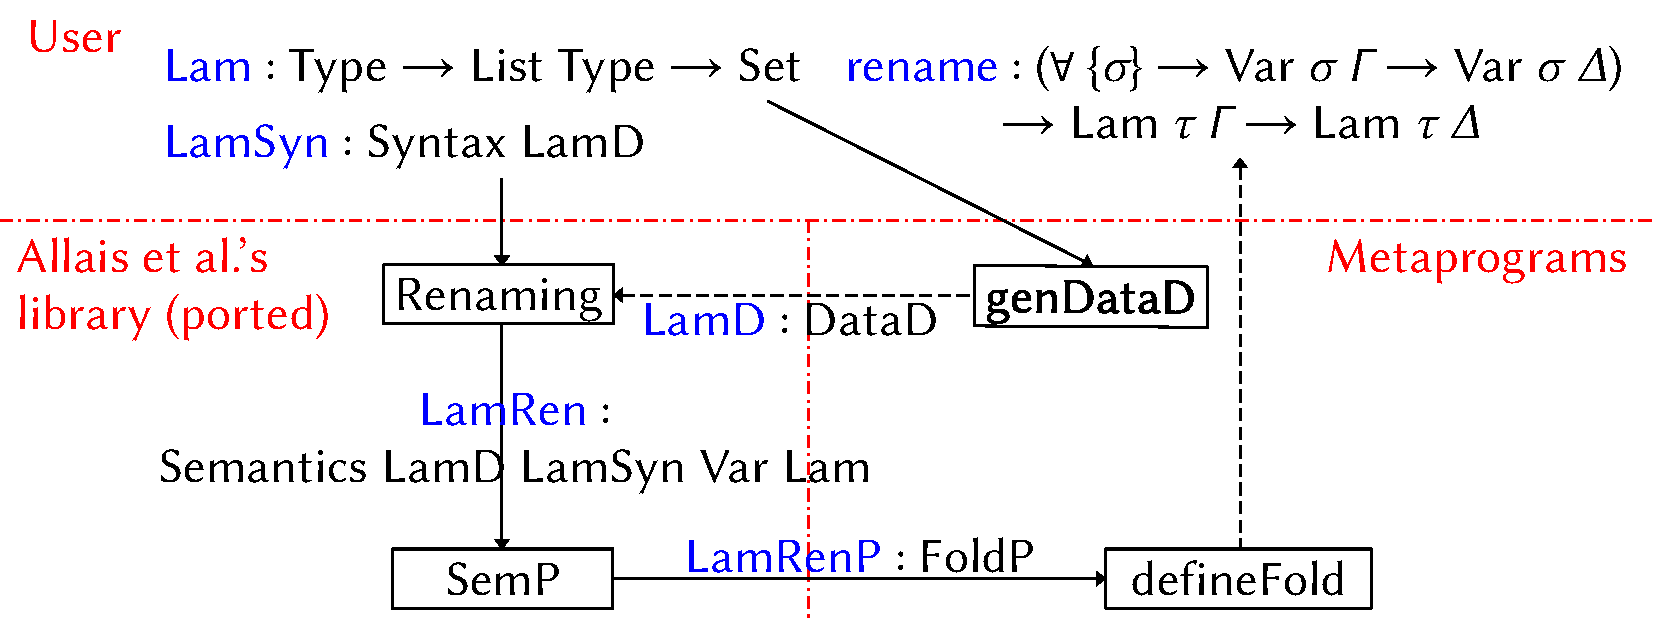
\includegraphics[width=\columnwidth]{Diagram.pdf}
\end{frame}

\begin{frame}[fragile]{The \mi{Syntax} Predicate}
\mi{Syntax}, a predicate on \mi{DataD}, captures datatypes that are syntaxes in \mi{Desc}.
	\begin{hscode}\SaveRestoreHook
\column{B}{@{}>{\hspre}l<{\hspost}@{}}%
\column{E}{@{}>{\hspre}l<{\hspost}@{}}%
\>[B]{}\Conid{Syntaxᵈ}\;\mathbin{:}\;\Conid{Set}\;\Varid{ℓ}\;\Varid{→}\;\Conid{DataD}\;\Varid{→}\;\Conid{Setω}{}\<[E]%
\ColumnHook
\end{hscode}\resethooks
\end{frame}

\begin{frame}[fragile]{The \mi{Syntax} Predicate}
Let's specify what syntaxes are captured by \mi{Desc}:
	\begin{itemize}
		\item each of them has a variable rule as its first rule,
		\item they are not universe polymorphic,
		\item each have two indices, $I$ and $\mi{List}\ I$, and
		\item allow and only allow context extensions in subterms.
	\end{itemize}
There's a catch: \mi{DataD} satisfying \mi{Syntax} is not isomorphic to \mi{Desc}!
\end{frame}

\begin{frame}[fragile]{The \mi{Syntax} Predicate}
Does \mi{PCF} satisfies \mi{Syntax}?
	\begin{hscode}\SaveRestoreHook
\column{B}{@{}>{\hspre}l<{\hspost}@{}}%
\column{3}{@{}>{\hspre}l<{\hspost}@{}}%
\column{10}{@{}>{\hspre}l<{\hspost}@{}}%
\column{27}{@{}>{\hspre}l<{\hspost}@{}}%
\column{E}{@{}>{\hspre}l<{\hspost}@{}}%
\>[B]{}\mathbf{data}\;\Conid{PCF}\;\mathbin{:}\;\Conid{Type}\;\Varid{→}\;\Conid{List}\;\Conid{Type}\;\Varid{→}\;\Conid{Set}\;\mathbf{where}{}\<[E]%
\\
\>[B]{}\hsindent{3}{}\<[3]%
\>[3]{}\Varid{‵var}\;{}\<[10]%
\>[10]{}\mathbin{:}\;\Conid{Var}\;\Varid{σ}\;\Conid{Γ}\;\Varid{→}\;\Conid{PCF}\;\Varid{σ}\;\Conid{Γ}{}\<[E]%
\\
\>[B]{}\hsindent{3}{}\<[3]%
\>[3]{}\Varid{‵app}\;{}\<[10]%
\>[10]{}\mathbin{:}\;\Conid{PCF}\;(\Varid{σ}\;\Varid{‵→}\;\Varid{τ})\;\Conid{Γ}\;\Varid{→}\;\Conid{PCF}\;\Varid{σ}\;\Conid{Γ}\;\Varid{→}\;\Conid{PCF}\;\Varid{τ}\;\Conid{Γ}{}\<[E]%
\\
\>[B]{}\hsindent{3}{}\<[3]%
\>[3]{}\Varid{‵lam}\;{}\<[10]%
\>[10]{}\mathbin{:}\;\Conid{PCF}\;\Varid{τ}\;(\Varid{σ}\;\Varid{∷}\;\Conid{Γ})\;{}\<[27]%
\>[27]{}\Varid{→}\;\Conid{PCF}\;(\Varid{σ}\;\Varid{‵→}\;\Varid{τ})\;\Conid{Γ}{}\<[E]%
\\
\>[B]{}\hsindent{3}{}\<[3]%
\>[3]{}\Varid{‵zero}\;{}\<[10]%
\>[10]{}\mathbin{:}\;\Conid{PCF}\;\Varid{‵ℕ}\;\Conid{Γ}{}\<[E]%
\\
\>[B]{}\hsindent{3}{}\<[3]%
\>[3]{}\Varid{‵suc\char95 }\;{}\<[10]%
\>[10]{}\mathbin{:}\;\Conid{PCF}\;\Varid{‵ℕ}\;\Conid{Γ}\;\Varid{→}\;\Conid{PCF}\;\Varid{‵ℕ}\;\Conid{Γ}{}\<[E]%
\ColumnHook
\end{hscode}\resethooks
\end{frame}

\begin{frame}[fragile]{The Syntax Predicate}
	\metroset{block=fill}
	\begin{exampleblock}{A Syntax proof example}
		\begin{hscode}\SaveRestoreHook
\column{B}{@{}>{\hspre}l<{\hspost}@{}}%
\column{9}{@{}>{\hspre}l<{\hspost}@{}}%
\column{E}{@{}>{\hspre}l<{\hspost}@{}}%
\>[B]{}\Conid{SyntaxPCF}\;\mathbin{:}\;\Conid{Syntaxᵈ}\;\Conid{Type}\;(\Varid{genDataD}\;(\Varid{quote}\;\Conid{PCF})){}\<[E]%
\\
\>[B]{}\Conid{SyntaxPCF}\;\mathrel{=}\;\anonymous \;{}\<[E]%
\\
\>[B]{}\hsindent{9}{}\<[9]%
\>[9]{}\Varid{,}\;\Varid{refl}\;{}\<[E]%
\\
\>[B]{}\hsindent{9}{}\<[9]%
\>[9]{}\Varid{,}\;(\Varid{refl}\;\Varid{,refl})\;{}\<[E]%
\\
\>[B]{}\hsindent{9}{}\<[9]%
\>[9]{}\Varid{,}\;\anonymous \;{}\<[E]%
\\
\>[B]{}\hsindent{9}{}\<[9]%
\>[9]{}\Varid{,}\;\Varid{refl}\;{}\<[E]%
\\
\>[B]{}\hsindent{9}{}\<[9]%
\>[9]{}\Varid{,}\;\Varid{refl}\;{}\<[E]%
\\
\>[B]{}\hsindent{9}{}\<[9]%
\>[9]{}\Varid{,}\;(\anonymous \;\Varid{,}\;\anonymous \;\Varid{,}\;\anonymous \;\Varid{,}\;\Varid{refl}\;\Varid{,}\;(\Varid{λ}\;\anonymous \;\Varid{→}\;\Varid{refl}))\;{}\<[E]%
\\
\>[B]{}\hsindent{9}{}\<[9]%
\>[9]{}\Varid{,}\;(\anonymous \;\Varid{,}\;\anonymous \;\Varid{,}\;\anonymous \;\Varid{,}\;\Varid{refl}\;\Varid{,}\;(\Varid{λ}\;\anonymous \;\Varid{→}\;\Varid{refl}))\;{}\<[E]%
\\
\>[B]{}\hsindent{9}{}\<[9]%
\>[9]{}\Varid{,}\;(\anonymous \;\Varid{,}\;\anonymous \;\Varid{,}\;\anonymous \;\Varid{,}\;\Varid{refl}\;\Varid{,}\;(\Varid{λ}\;\anonymous \;\Varid{→}\;\Varid{refl}))\;{}\<[E]%
\\
\>[B]{}\hsindent{9}{}\<[9]%
\>[9]{}\Varid{,}\;(\anonymous \;\Varid{,}\;\anonymous \;\Varid{,}\;\anonymous \;\Varid{,}\;\Varid{refl}\;\Varid{,}\;(\Varid{λ}\;\anonymous \;\Varid{→}\;\Varid{refl}))\;{}\<[E]%
\\
\>[B]{}\hsindent{9}{}\<[9]%
\>[9]{}\Varid{,}\;\Varid{tt}{}\<[E]%
\ColumnHook
\end{hscode}\resethooks
	\end{exampleblock}
	\mi{Syntax} proofs in this case are amenable to be generated with elaborator reflection.
\end{frame}

% \begin{frame}[fragile]{Translation from Semantics to natural looking functions}
% \end{frame}

\section{Demo}

\section{Discussion}

\begin{frame}[fragile]{Towards datatype-generic libraries for all syntaxes?}
\end{frame}

\end{document}

